%%%%%%%%%%%%%%%%%%%%%%% file template.tex %%%%%%%%%%%%%%%%%%%%%%%%%
% This is a general template file for the LaTeX package SVJour3
% for Springer journals.          Springer Heidelberg 2006/03/15
% Copy it to a new file with a new name and use it as the basis
% for your article. Delete % signs as needed.
% This template includes a few options for different layouts and
% content for various journals. Please consult a previous issue of
% your journal as needed.
%%%%%%%%%%%%%%%%%%%%%%%%%%%%%%%%%%%%%%%%%%%%%%%%%%%%%%%%%%%%%%%%%%%
% First comes an example EPS file -- just ignore it and
% proceed on the \documentclass line
% your LaTeX will extract the file if required
%\begin{filecontents*}{example.eps}
%!PS-Adobe-3.0 EPSF-3.0
%%BoundingBox: 19 19 221 221
%%CreationDate: Mon Sep 29 1997
%%Creator: programmed by hand (JK)
%%EndComments
%gsave
%newpath
%  20 20 moveto
%  20 220 lineto
%  220 220 lineto
%  220 20 lineto
%closepath
%2 setlinewidth
%gsave
%  .4 setgray fill
%grestore
%stroke
%grestore
%\end{filecontents*}
%\documentclass{svjour3}                    % onecolumn (standard format)
%\documentclass[smallextended]{svjour3}     % onecolumn (second format)
\documentclass[twocolumn]{svjour3}          % twocolumn
%\smartqed  % flush right qed marks, e.g. at end of proof
\usepackage{graphicx}
\usepackage{mathptmx} % use Times fonts if available on your TeX system
% insert here the call for the packages your document requires
\usepackage{latexsym}
% etc.
% please place your own definitions here and don't use \def but
% \newcommand{}{}
% Insert the name of "your journal" with
\journalname{Innovations in Systems and Software Engineering}
%%%%%%%%%%%%%%%%%%%%%%%%%%%%%%%%%%%%%%%%%%%%%%%%%%%%%%%%%%%%%
\begin{document}

\title{URDAD as a Semi-Formal Approach to Analysis and Design\thanks{This
	paper is part of an ongoing PhD project by Fritz Solms under the supervision
	of Stefan Gruner at the Department of Computer Science of the University of
	Pretoria. We would like to thank Stefan Gruner for the fruitful discussions 
	we had on this topic.}}
	
\titlerunning{URDAD} % if too long for running head
\author{Fritz Solms \& Dawid Loubser}
\authorrunning{Solms/Loubser} % if too long for running head

\institute{F. Solms \at
              Dept. Computer Science \\
              University of Pretoria \\
              Republic of South Africa \\
              \email{fritz@solms.co.za}}

\date{Received: \today / Accepted: date}
% The correct dates will be entered by the editor

\maketitle

\begin{abstract}
The Use Case, Responsibility Driven Analysis and Design (URDAD) methodology, is
a methodology for technology neutral design generating the Platform Independent
Model (PIM) of the Object Management Group's (OMG's) Model Driven Architecture (MDA).
It requires the core modeling to be done in the problem space by
domain specialists and not in the solution space by technology specialists.
URDAD allows for formal elements to be
added by different role players at different stages of the model refinement,
whilst aiming to preserve agility of the outputs and low cost of the process
generating the outputs.
This paper discusses the semi-formal aspects of URDAD
which facilitate model validation and testing, documentation
generation and automated implementation mapping as well as those
which promote agility and low cost.
\keywords{URDAD Method, Formal Methods, Agile Processes}
%%%%%%%%%%%%%%%%%%%%%%%%%% \PACS{PACS code1 \and PACS code2 \and more}
%%%%%%%%%%%%%%%%%%%%%%%% \subclass{MSC code1 \and MSC code2 \and more}
\end{abstract}

\section{Introduction}
\label{sec:introduction}
Formal methods aim to provide non-ambiguous requirements and a design
which can be proven to be correct and reliable \cite{Monin:understandingFormalMethods}.
These methods are, however, perceived as difficult and expensive: their
use has largely been confined to a relatively small class of problems
where safety and reliability are paramount (such as the aviation \cite{hall:formalMethodsInRealAirTraffic}
and defense industries, where testing and debugging costs can contribute more
than 50\% of the development costs
\cite{platzer:verificationOfCyberphysicalTransportationSystems}.)

Agile methods \cite{agileManifesto,martin:agileSoftwareDevelopment},
on the other hand accept that the initial requirements are potentially
incomplete, partially incorrect and volatile. They aim to provide a process which
can operate successfully within such an environment. Modeling is seen
largely as a tool used to facilitate domain exploration and simplification
of the solution whilst the primary output of the process is working code.

Model-driven development (MDD)
\cite{stahl:mdsd,france:mddUsingUml2} has been
influenced by both, formal \cite{oquendo:modelDrivenFormalMethod}
and agile \cite{lazar:agileMdaForSoa,solms:generatingMdasPimUsingUrdad}
methods. The formal approach is
required for model transformation and code generation. The agile aspect
is important for business and system agility, i.e.\ to cost effectively
address requirements evolution. 

The OMG's vision of MDD is MDA \cite{siegel:developingInMDA}.
It is supported by an elaborate technology suite including support for modeling
via the Unified Modeling Language (UML), meta language specification via the
Meta-Object Facility (MOF), model querying and constraint specification and
transformation via the object constraint language (OCL) and the 
Query/View/Transformations (QVT) specification. MDA aims to provide a level of agility whilst being
sufficiently formal to be able to automate large parts of the implementation 
mapping 
by enabling domain experts to perform a semi-formal analysis and design
in UML which can then be incrementally formalized through model refinement
and the use of OCL.


The value obtained from MDA based projects has been limited by
\cite{solms:generatingMdasPimUsingUrdad}
\begin{itemize}
  \item the lack of standards for specifying the implementation architecture and technologies,
  \item the lack of a well-defined analysis and design methodology used to generate
the platform independent model (PIM), as well as 
  \item the wide variation in model structure and content permitted by the UML, increasing
the complexity of the implementation mapping.
\end{itemize}

Various attempts have been made to both simplify and increase the formality of UML models by
restricting the number of diagrams and UML elements used and adding formal specification
techniques to the UML model.
\cite{Bruel:integratingFormalAndInformalSpecificationTechniques,mccumber:generalFrameworkForFormalinzingUmlWithFormalLanguages}. 
URDAD similarly restricts the use of UML
constructs to a small but sufficient subset of UML, and enforces a 
specific model structure with specified model elements. 
However, with the availability and growing
support for the OCL a lot the formalization is done within UML and OCL. 

A number of service oriented design methodologies have been proposed
\cite{Moosavi:methodForServiceOrientedDesign,ma:mddPlatformForSoa}.
\cite{ma:mddPlatformForSoa}, like URDAD, integrates the services oriented approach within a 
model-driven approach. Many of these services oriented design methodologies use BPMN
and often these approaches are technology specific. URDAD aims to provide
a more formal, technology neutral approach based on the use of UML and
OCL. OCL is used to formalize both, the contract and process specifications.
This semi-formal approach facilitates model validation and transformation including
documentation and code generation.

In this paper we point out the semi-formal aspects of URDAD facilitating model validation,
automated generation of functional testing, documentation generation and simplified implementation mapping as well as aspects of an URDAD model and approach which improve agility.

%%%%%%%%%%%%%%%%%%%%%%%%%%%%%%%%%%%%%%%%%%%%%%%%%%%%%%%%

\section{URDAD}
\label{sec:urdad}

URDAD
\cite{solms:generatingMdasPimUsingUrdad,solms:urdad}
is a service-oriented analysis and design methodology. A number
of organizations, particularly in the financial and insurance
sectors, have adopted this methodology for their technology 
neutral business process design  
\cite{klopper:compareSoftwareMethodologies}.
It aims to provide a simple repeatable engineering process for
generating MDA's PIM. The repeatability aspect aims to ensure that the
outputs from different domain experts with similar
domain knowledge would be very similar. To achieve this,
URDAD provides a step-for-step process for analysing and
designing the technology neutral solution with well defined inputs
and outputs for each step.

%=============================

\subsection{The methodology}

Instead of following a waterfall approach within a particular service/use case, 
(i.e. peforming analysis, design, implementation, testing and deployment for each use case)
URDAD requires that
one performs analysis and design across levels of granularity. This is illustrated in figure
\ref{fig:urdadHighLevel} which shows that for any use case, the high-level requirements analysis
and formalization within a services contract is followed by a design which assembles a process
realizing the higher level service from lower level services.The analysis and design for those
lower level services is done as one traverses to the next lower level of granularity.

\begin{figure}[ht!]
  \begin{center}
    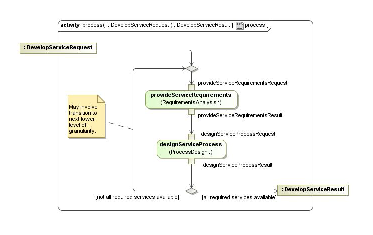
\includegraphics[width=8cm]{urdadHighLevel}
    \caption{\it High-level view of URDAD showing analysis and design across levels of granularity.}
    \label{fig:urdadHighLevel}
  \end{center}
\end{figure}

Services are recursively constructed from lower level services
with the lowest level services being either not domain specific 
(generic services like numeric addition, or infrastructure services 
such as persistence) or services which are sourced externally. 
These externally-sourced services are treated as a black box, 
but the methodology still requires the specification of a full 
services contract.
Figure \ref{fig:urdadHighLevel} also points out that one terminates the 
analysis and design as soon as all required services are available.

One of the core aspects of URDAD is that it requires analysis
and design to be done across levels of granularity, with both
of these done by domain experts from different specialization
areas. Thus instead of requiring a (business) analyst
to specify the entire requirements for a new service,
this responsibility is distributed across domain experts of
domains touched by the service requirements.

For example, the business
process for processing an insurance claim may require services
for assessing the claim coverage and value, as well as for
settling the claim and recuperating any losses. Those are
very different responsibility domains and it is unreasonable
to expect a business analyst to be able to provide the detailed
requirements for a business process across levels of
granularity. Instead a business analyst from claims could specify the high-level 
requirements (such as that the losses need to be recuperated)
without having to specify the detailed requirements and process
for those lower level services. He/she is assembling the higher
level business process across level services sourced from other
domains of responsibility whose detailed requirements and designs
are done by domain experts from those domains of responsibility.

%=======================================================

\subsection{The analysis phase}

Figure \ref{fig:urdadAnalysis} shows the steps for the URDAD analysis phase.
URDAD requires that one first identifies the stakeholders
which have an interest in and hence requirements for the use case/service. These
are represented as interfaces. 
\footnote{URDAD uses interfaces for roles. Like actors, interfaces
conceptually represent roles. Actors are, however, problematic as the object may or may not
be external depending on the level of granularity and because UML actors cannot absorb 
any service requirements. For example, a user may have to do certain things when
using a service. Using interfaces enables us to absorb these service requirements
for external objects in a contract for that role.}


\begin{figure}[ht!]
  \begin{center}
    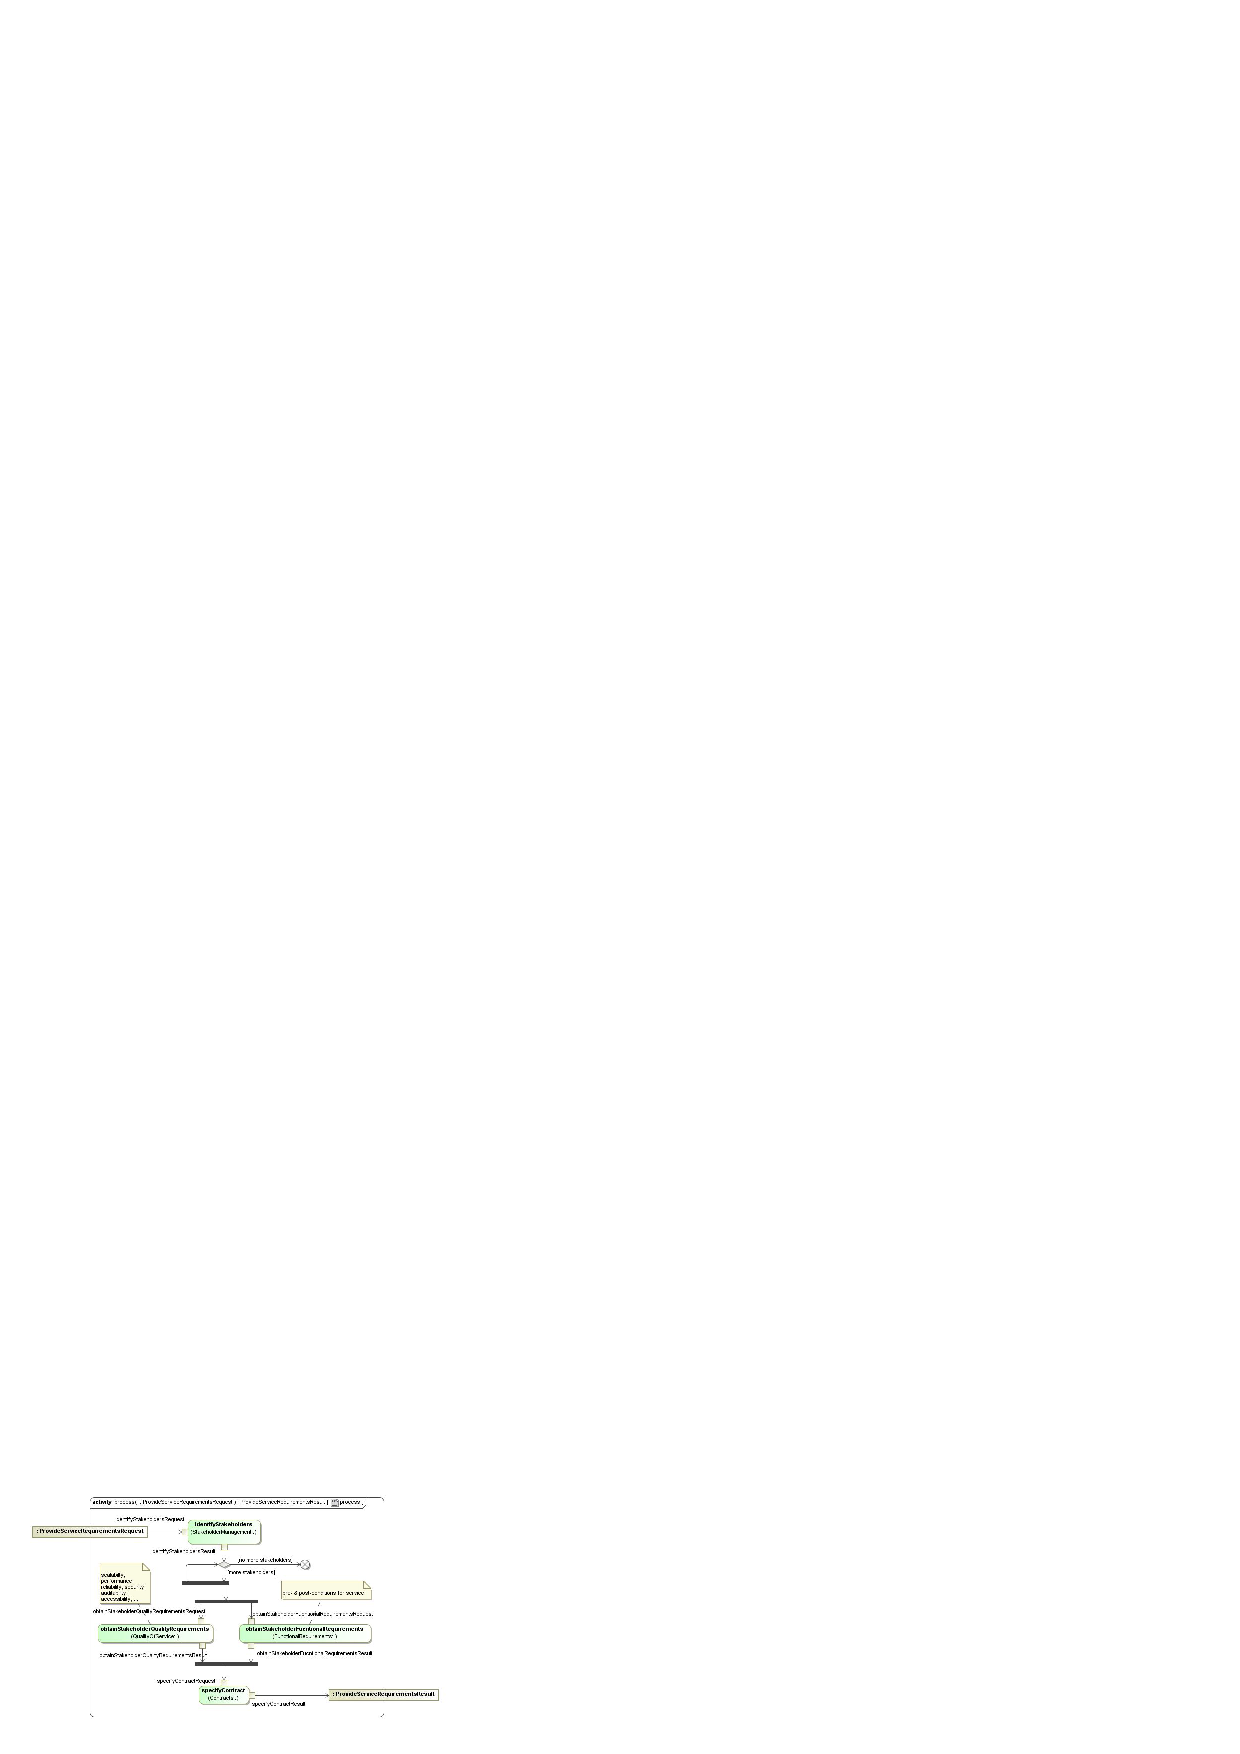
\includegraphics[width=8cm]{urdadAnalysis}
    \caption{\it The steps for the analysis phase of URDAD.}
    \label{fig:urdadAnalysis}
  \end{center}
\end{figure}


Next one identifies the pre- and post-conditions as well
as quality requirements the different stakeholders have for the service. As these
are independent, this can be done concurrently. The aggregated service requirements 
for the current level of granularity are ultimately encapsulated in a contract for
the service which is visually represented in UML as a class diagram.
Initially the domain experts may specify the pre- and post-conditions and quality
requirements in English. These are incrementally formalized by mapping the pre-
and post-conditions onto OCL  and the quality requirements onto the UML Quality of
Service (QOS) profile \cite{omg:qualityOfService}.

A simplified example of such a class diagram is shown in figure 
\ref{fig:servicesContract}.

\begin{figure}[ht!]
  \begin{center}
    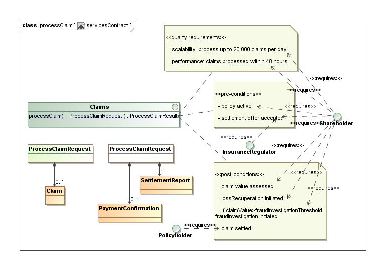
\includegraphics[width=8cm]{servicesContract}
    \caption{\it A simplified services contract for a process claim use case.}
    \label{fig:servicesContract}
  \end{center}
\end{figure}

Note that URDAD requires the linkage between stakeholders and their functional and non-functional
requirements via \verb+<<requires>>+ dependencies in the UML model maintaining the information on
who requires what.

URDAD also requires that there is a single request and a single result object for each service. This
improves understandability and maintainability, avoiding scenarios where change requests result in
direct interface changes and potentially in long, sparsely populated parameter lists with different
scenarios requiring different sets of parameteres to be provided. The data structure for the result
object is populated from the user requirements. The data structure for the request object is, however,
initially left blank and is incrementally populated as one does the design across levels of granularity 
and identifies the need for certain information in order to render the required service.

%=======================================================

\subsection{The design phase}

The steps for the design phase of URDAD are shown in  \ref{fig:urdadHighLevel}.
One first identifies the services required for the enforcement of each pre- and post-condition.
Next one tries to group services into cohesive, higher-level services. This is required to fix 
the level of granularity in a repeatable way. One then assigns services to separate services
contracts. Finally one assembles the process realizing the service from these lower level services.

\begin{figure}[ht!]
  \begin{center}
    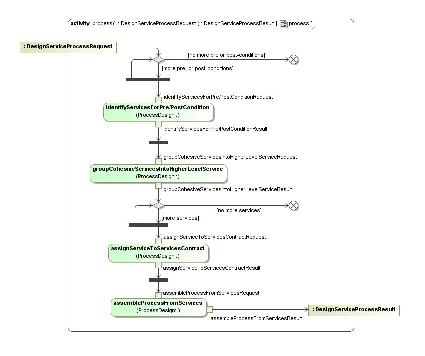
\includegraphics[width=8cm]{urdadDesign}
    \caption{\it The steps for the analysis phase of URDAD.}
    \label{fig:urdadDesign}
  \end{center}
\end{figure}

The URDAD model can be populated through the use of only two UML diagrams,
a class diagram for the required
services and the services contracts to which these services are assigned, and an activity diagram
for the process specification.


\begin{figure}[ht!]
  \begin{center}
    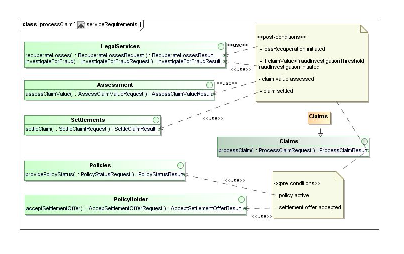
\includegraphics[width=8cm]{serviceRequirements}
    \caption{\it The service requirements and responsibility allocation step.}
    \label{fig:serviceRequirements}
  \end{center}
\end{figure}

The service requirements diagram shows the services used to realize the various pre- and 
post-condition as well as the services contracts to which these services have been assigned.

The process specification shows how the process is assembled across services sourced from the
various service providers.

\begin{figure}[ht!]
  \begin{center}
    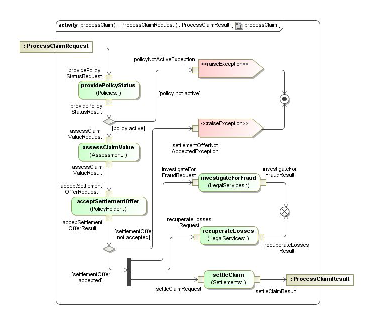
\includegraphics[width=8cm]{processClaim}
    \caption{\it Process specification for process claim service.}
    \label{fig:processClaim}
  \end{center}
\end{figure}



%=======================================================

\subsection{UML concerns}

URDAD requires the linkage between stakeholders and their requirements 
(pre- and post-conditions and quality requirements) via \verb+requires+
dependencies (the \verb+<<requires>>+ stereotype is defined in an URDAD 
profile) as well as the linkage between
pre- and post-conditions and the services required to address them via
standard UML \verb+<<uses>>+ dependencies. Whilst this is all fine within the
UML model, the UML specification does not specify any standard notation
for rendering constraints like pre- and post-conditions. The support for
rendering constraints is thus tool dependent and may be non-existent.
This defficiency may require domain specialists to insert the dependency
relationships at the model level.

%%%%%%%%%%%%%%%%%%%%%%%%%%%%%%%%%%%%%%%%%%%%%%%%%%%%%%%%%%%%%%%%%%%%%%%%%%%%

\section{Semi-formal elements of URDAD}
\label{sec:semiFormalElements}

Two aspects of URDAD introduce a level of formality on the model. Firstly it is the 
requirement that the 
requirements for any service are specified as a formal services contract from which tests which
assess whether any designed or implemented service fulfills the contract. The second aspect
of URDAD is the
formal definition of the URDAD model structure and content which is verifiable through a model 
validation suite.




%Formal methods \cite{Monin:understandingFormalMethods, hinchey:softwareEngineeringAndFormalMethods}
%are precise, mathematically
%rigorous methods which remove ambiguity and result in verifiable implementations.
%The three core approaches are based on denotational, operational
%and axiomatic semantics.

%In both denotional and operational semantics, one defines the meaning of what the
%program represents/does. These approaches provide the ability to formally prove
%an algorithm. For complex problems the approach may, however, be very costly.
%Furthermore, there could be multiple algorithms which could suitably realize the stakeholder's
%requirements - yet one will lock into a particular algorithm which
%can potentially be proven correct, but which may not be the best with respect to certain
%quality requirements like simplicity, performance, resource-efficiency (e.g. memory
%efficiency, ...) and so on. Furthermore, replacing one algorithm with another is a complex task
%which typically requires a complete redefinition of the algorithm and its proofs, and
%may have a wide ranging impact across the system.

%=======================================

\subsection{Formal contracts-based approach}

Since the model should preferably be developed in the problem/requirements domain and not in the
technical/solution domain, an axiomatic/contracts based approach is natural to 
model-driven development
\cite{Briand:investigationOfFormalityInUmlBaedDevelopment}. URDAD uses this formal contracts based approach, facilitating
the auto-generation of algorithm-independent tests
\cite{meyer:programsThatTestThemselves}. 
This is done recursively,
by assuming at any particular level of granularity, that the lower level services used within
the algorithm do realize their respective services contracts.

%====================================


\subsection{Well defined, verifiable model structure}

In addition to the service contracts across levels of granularity, URDAD enforces a number
of other elements which formalize the outputs of the methodology including
\begin{itemize}
  \item an OCL validation suite which validate that the UML model complies to the
			constraints of an URDAD meta-model, and
  \item OCL validation suites for model completeness and consistency.
\end{itemize}

These validation suites enforce
\begin{itemize}
  \item the linking of pre- and post-conditions to functional/service
			requirements (use cases) through which these pre- and post-conditions are
			addressed,
	\item the linking of functional requirements (use cases) to services
			in services contracts which formalize the service requirements,
	\item the linking of service process specifications to the service contracts they realize,
	\item the construction of request objects for each service
			from the information available to the (business) process at the
			stage of service request,
	\item the construction of result objects from the information available
			at the end of the process realizing the service,
	\item the specification of contracts for all role players
			including users and service providers across levels of granularity,
	\item that for each pre-condition a corresponding exception is raised,
			informing the user that the service requested is not going to be provided.
			All other scenarios satisfying the pre-conditions for the service
			lead to the provision of the result object.
\end{itemize}
The first three provide bi-directional requirements traceability. Black-box
tests can be auto-generated from the services contracts.

Note that if the levels of granularity are not carefully managed,
the specification of some of the above constraints can become very complex. The
methodology, however, aims to provide a repeatable algorithm through which the levels
of granularity are fixed in a way which minimizes complexity at any particular level
of granularity, and which maximizes re-use of services.

The validation suites enforces a complete, consistent model which has sufficient
information to facilitate a complete implementation mapping. The details for the
implementation architecture and technologies need to be provided separately.

%=============================

\subsection{Incremental formalization of model}


The requirements specification in the form of formal contracts using the OCL is, however, non-trivial.
It is generally not feasible to expect domain specialists like business analysts to specify  
formal services contracts. URDAD allows for domain experts to specify
services contracts informally (using natural language to specify constraints, for example), 
with OCL experts subsequently mapping such statements onto OCL. 

In order to automate the full code generation, OCL experts will have to formalize the guard conditions
as well as how request objects are to be constructed from the information available to the process.

%%%%%%%%%%%%%%%%%%%%%%%%%%%%%%%%%%%%%%%%%%%%%%%%%%%%%%%%%%%%%%%%%%%

\section{What makes an URDAD based approach agile?}
\label{sec:urdadAgility}

Agile approaches
\cite{martin:agileSoftwareDevelopment,agileManifesto}
like Extreme Programming \cite{beck:extremeProgrammingExplained2}
accept and even welcome continuously changing requirements in the
context of continuously changing business opportunities and
continuous growth of knowledge on how to improve stake
holder value generation. They aim to be able to provide better business value
by being able to effectively operate in an environment of
continuously changing requirements.

In such a high-risk environment it is critical to manage and mitigate
risk. This is done through practices like short feedback cycles
via short releases, on-site customer, pair-programming,
enforced, automated functional (unit) testing across levels of
granularity, and continuous integration testing.

Agile methodologies typically handle the removal of any unnecessary complexity
arising from an agile approach through peer reviews and continuous refactoring
facilitated through non-ownership of all artifacts generated by the process.

%------------------------------------------------------------------

\subsection{Applying agile principles and practices in MDD}

MDD decouples the requirements and design from the implementation architecture
and technologies and increases the level of abstraction of development.
However, continuously changing requirements are core to business agility.
Many of the agile practices have been ported to this higher level of abstraction
including on-site customer (with the customer communication simplified
as the design is done in the problem/business domain), pair design,
enforced and automated functional testing at the design level either via
proving the design or executing the design in model execution environments
\cite{kirshin:umlGenericModelExecutionEngine},
peer reviews and non-ownership of designs.

In addition, MDD, and MDA in particular, aim to improve agility around technology
and architecture by decoupling the design from these and automating the
implementation mapping onto the target architecture and technologies.

%------------------------------------------------------------------

\subsection{How does URDAD aim to achieve agility?}

URDAD itself is not a development process but a process for performing
the technology neutral analysis and design generating MDA's PIM. It is
typically embedded within a model-driven development process within
which some of the agile principles and practices can be absorbed. 

However, the URDAD methodology aims to increase
agility through a number of intrinsic process elements
\begin{itemize}
  \item enforced decoupling across all levels of granularity, facilitated
			through enforced binding to services contracts, implied adapters
			to concrete service providers and localization of process in
			separate work flow controllers,
  \item explicit search step for service reuse resulting in lower cost and complexity reduction, 
  \item automated documentation (including UML to natural language mapping
			and UML diagram generation) from the URDAD compliant UML model, and
  \item complexity reduction through enforced responsibility localization.
  \item rapid informal contract and design specification by domain specialists followed by
incremental formalization of the design by technical specialists.
\end{itemize}

%%%%%%%%%%%%%%%%%%%%%%%%%%%%%%%%%%%%%%%%%%%%%%%%%%%%%%%%%%%%%%%%%%%%%%%%%%%%%%%%%%

\section{Conclusions and outlook}
\label{sec:conclusions}

Over the years URDAD has strengthened its formal aspects through the introduction of model validation
and formal model structure specification as well as the use of OCL to formalize the contracts specification.
This has simplified model testing and transformation tasks like documentation generation and 
implementation mappings.

However, using standard UML modeling tools results in a lot of unnecessary overheads for modelers who 
have to construct the appropriate URDAD model structure themselves, obtaining only guidelines from 
the results of the model validations. The agility of URDAD can be considerably improved by
\begin{itemize}
  \item developing an URDAD front-end to UML which enforces the URDAD model structure directly and 
which guides modelers explicitly through the URDAD process, 
  \item extending the range of documentation generation transformations to provide suitable 
model views for different role players, and
  \item developing URDAD specific implementation mapping transformations for widely used 
implementation technologies in infrastructures.
\end{itemize}

%%%%%%%%%%%%%%%%%%%%%%%%%%%%% BibTeX users please use one of
%\bibliographystyle{spbasic}% basic style, author-year citations
%\bibliographystyle{spmpsci}% mathematics and physical sciences
%\bibliographystyle{spphys} % APS-like style for physics
%\bibliography{}            % name your BibTeX data base
% Non-BibTeX users please use %%%%%%%%%%%%%%%%%%%%%%%%%%

\begin{thebibliography}{}

\bibitem{beck:extremeProgrammingExplained2}
Kent Beck and Cynthia Andres.
\newblock {\em Extreme Programming Explained}.
\newblock Addison-Wesley Professional, second edition, 2004.

\bibitem{agileManifesto}
Kent Beck, Martin Fowler, Robert~C. Martin, et~al.
\newblock The agile manifesto.
\newblock http://agilemanifesto.org/, 2001.

\bibitem{Briand:investigationOfFormalityInUmlBaedDevelopment}
L.C. Briand, Y.~Labiche, M.~{Di Penta}, and H.~Yan-Bondoc.
\newblock An experimental investigation of formality in uml-based development.
\newblock {\em Software Engineering, IEEE Transactions on}, 31(10):833--849,
  Oct. 2005.

\bibitem{Bruel:integratingFormalAndInformalSpecificationTechniques}
J.-M.~ Bruel, B.~ Cheng, S.~ Easterbrook, R.~ France and B.~ Rumpe
\newblock Integrating formal and informal specification techniques. why? how?
\newblock In {\em 2nd IEEE Workshop on Industrial Strength Formal Specification Techniques, 1998. Proceedings.},
   pages 50--57.

\bibitem{hall:formalMethodsInRealAirTraffic}
A.~Hall and D.~Isaac.
\newblock Software in air traffic control systems.
\newblock In {\em The Future, IEE Colloquium on}, pages 7/1--7/4, Jun 1992.

\bibitem{hinchey:softwareEngineeringAndFormalMethods}
Mike Hinchey, Michael Jackson, Patrick Cousot, Byron Cook, Jonathan~P. Bowen,
  and Tiziana Margaria.
\newblock Software engineering and formal methods.
\newblock {\em Commun. ACM}, 51(9):54--59, 2008.

\bibitem{kirshin:umlGenericModelExecutionEngine}
Andrei Kirshin, Dolev Dotan, and Alan Hartman.
\newblock {\em A UML Simulator Based on a Generic Model Execution Engine},
  volume 4364/2007 of {\em Lecture Notes in Computer Science}, pages 324--6.
\newblock Springer, Berlin / Heidelberg, 2007.

\bibitem{klopper:compareSoftwareMethodologies}
Riaan Klopper, Stefan Gruner, and Derrick Kourie.
\newblock Assessment of a framework to compare software development
  methodologies.
\newblock In {\em Proceedings of the 2007 annual research conference of the
  South African institute of computer scientists and information technologists
  on IT research in developing countries}, volume 226 of {\em ACM International
  Conference Proceeding Series}, pages 56--65. ACM Press, 2007.

\bibitem{lazar:agileMdaForSoa}
I.~Lazar, B.~Parv, S.~Motogna, I.-G. Czibula, and C.-L. Lazar.
\newblock An agile mda approach for the development of service-oriented
  component-based applications.
\newblock In {\em CANS '08: Proceedings of the 2008 First International
  Conference on Complexity and Intelligence of the Artificial and Natural
  Complex Systems. Medical Applications of the Complex Systems. Biomedical
  Computing}, pages 38--44, Washington, DC, USA, 2008. IEEE Computer Society.

\bibitem{martin:agileSoftwareDevelopment}
Robert~C. Martin.
\newblock {\em Agile Software Development, Principles, Patterns, and
  Practices}.
\newblock Prentice-Hall, 2002.

\bibitem{mccumber:generalFrameworkForFormalinzingUmlWithFormalLanguages}
W.E.~ McCumber and B.H.C.~ Cheng
\newblock A general framework for formalizing UML with formal languages
\newblock In {\em Proceedings of the 23rd International Conference on Software Engineering}, 
 pages 433-442, 2001.

\bibitem{meyer:programsThatTestThemselves}
Bertrand Meyer, Arno Fiva, Ilinca Ciupa, Andreas Leitner, Yi~Wei, and Emmanuel
  Stapf.
\newblock Programs that test themselves.
\newblock {\em Computer}, 42(9):46--55, Sept. 2009.

\bibitem{Monin:understandingFormalMethods}
Jean~Francois Monin and Michael~Gerard Hinchey.
\newblock {\em Understanding formal methods}.
\newblock Springer, 2003.

\bibitem{Moosavi:methodForServiceOrientedDesign}
S.~ Moosavi, M.A.~ Seyyedi and N.~ Moghadam
\newblock {\em A Method for Service Oriented Design}
\newblock In Sixth International Conference on Information Technology: New Generations, 2009. ITNG '09.,
  pages 290-295, 2009.

\bibitem{omg:qualityOfService}
UML Profile for Modeling Quality of Service and Fault Tolerance Characteristics and Mechanisms.
\newblock document ptc/04-06-01, 2004.

\bibitem{oquendo:modelDrivenFormalMethod}
Flavio Oquendo.
\newblock Pi-method: a model-driven formal method for architecture-centric
  software engineering.
\newblock {\em SIGSOFT Softw. Eng. Notes}, 31(3):1--13, 2006.

\bibitem{platzer:verificationOfCyberphysicalTransportationSystems}
A.~Platzer.
\newblock Verification of cyberphysical transportation systems.
\newblock {\em Intelligent Systems, IEEE}, 24(4):10--13, July-Aug. 2009.

\bibitem{france:mddUsingUml2}
Sudipto Ghosh Trung Dinh-Trong {Robert B. France} and Arnor Solberg.
\newblock Model-driven development using {UML}-2: Promises and pitfalls.
\newblock {\em Computer}, 39(2):59--66, February 2006.

\bibitem{siegel:developingInMDA}
Jon Siegel.
\newblock Developing in {OMG}'s {M}odel-{D}riven {A}rchitecture.
\newblock White paper, Object Management Group, November 2001.

\bibitem{solms:urdad}
Fritz Solms.
\newblock Technology neutral business process design using {URDAD}.
\newblock In Hamido Fujita and Domenico Pisanelli, editors, {\em New Trends in
  Software Methodologies, Tools and Techniques}, Frontiers in Artificial
  Intelligence and Applications, pages 52--70. IOS Press, 2007.

\bibitem{solms:generatingMdasPimUsingUrdad}
Fritz Solms and Dawid Loubser.
\newblock Generating mda's platform independent model using urdad.
\newblock {\em Knowledge-Based Systems}, 22:174--185, 2009.

\bibitem{stahl:mdsd}
Thomas Stahl and Markus Voelter.
\newblock {\em Model-Driven Software Development}.
\newblock John Wiley \& Sons, 2004.

\bibitem{ma:mddPlatformForSoa}
Zhiyi Ma, Xiao He and Lianghuan Kang.
\newblock A Model Driven Development Platform for Service-Oriented Applications,
\newblock In World Conference on Services - II, 2009. SERVICES-2 '09, pages 17--24, 2009.


\end{thebibliography}
\end{document}
% end of file template.tex

